\chapter{Organisation}
Dette afsnit vil give et indblik i strukturen og opbygningen af Kvindeafdelingen, Svangre- og ultralydsambulatorium på Hospitalsenheden Horsens (HEH) og afdeling Kvindesygdomme og Fødsler på Regionshospitalet Midt Viborg (RMV). Afsnittet vil belyse, hvilken betydning implementeringen af en Ultralyds Robotarm, vil have for afdelingerne som organisation, samt hvilke ændringer dette vil medføre i arbejdsgangen for personalet. \\
Informationer, som er indhentet fra HEH og RMV, vil blive sammenholdt med videnskabelige artikler, i forsøget på at finde en større sammenhæng i problemstillingen omkring arbejdsgener ved ultralydsscanning. 

Det er valgt, at benyttes Leavitts organisationsmodel \ref{LeavittModel} som analysemetode. Denne model er en diamantmodel, der arbejder med fire organisatoriske hovedelementer, der relaterer sig til hinanden. Hvert hovedelement vil blive belyst i hvert sit underafsnit \cite{Leavitt}.

\begin{figure}[h!]\centering
	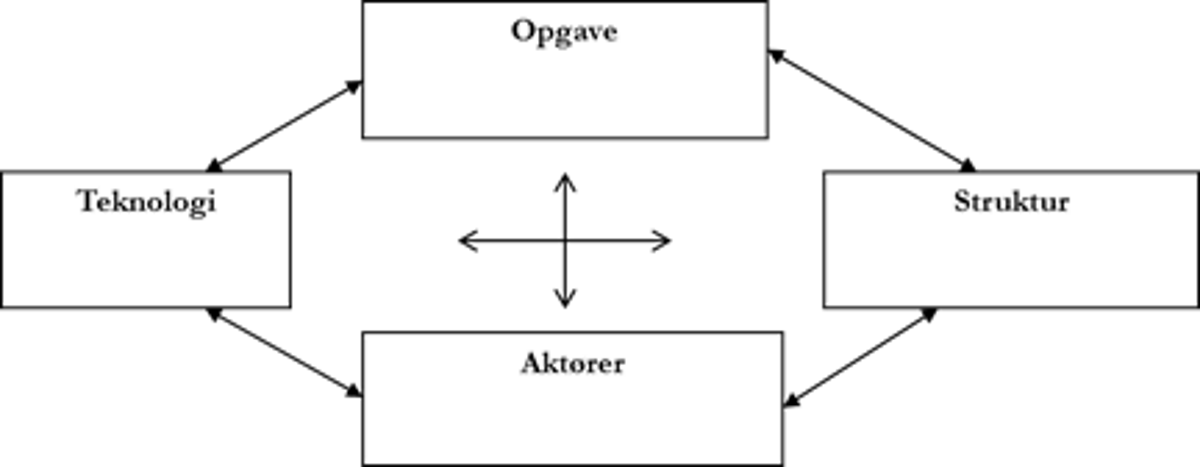
\includegraphics[width = 0.5\textwidth]{Figurer/LeavittModel}
	\caption{Leavitts organisationsmodel, viser hvordan struktur, aktører, opgaver og teknologi indbyrdes relaterer sig til hinanden, i midten haves kulturen for organisationen.}
	\label{LeavittModel}
\end{figure}
I analysen er der kun medtaget to ultralydsafdelinger, og derfor er der ikke videre empiri for at kunne drage konklusioner om, at billedet vil være det samme på andre lignende hospitals afdelinger i Danmark. 

Dataindsamlingen til analyse er indhentet gennem interview med afdelingssygeplejerske Tina Arnbjørn og tre sonografer fra HEH, samt interview med afdelingssygeplejerske Karen Marie Goul og en sonograf fra RMV.
Til at underbygge arbejdsskadeproblemstillingen benyttes yderligere videnskabelige artikler.

\section{Kvindeafdelingen, Svangre- og ultralydsambulatorium, Hospitalsenheden Horsens}
HEH er bemandet af en afdelingssygeplejerske, fem sonografer samt et ukendt antal læger. Afdelingen har udstyr til fire stuer, hvoraf tre stuer bemandes af sonografer. Der foretages 30-40 scanninger om dagen på afdelingen, hver scanning tager i gennemsnit 35 minutter.

\section{Kvindesygdomme og fødsler, Regionshospitalet Viborg}
Bemanding på RMV består af en afdelingssygeplejerske, ni sonografer og et ukendt antal læger. Afdelingen har ultralydsscanningsudstyr til fem stuer til gravide, hvoraf tre stuer er i drift dagligt og bemandes af sonografer. Dagligt foretages der 25-30 scanninger på afdelingen. En scanning tager i gennemsnittet 30 minutter.

Antallet af læger er ikke relevant for denne analyse, da der udelukkende fokuseres på sonografernes arbejdsgange.

\section{Leavitts organisationsmodel}
Det er valgt at sammenskrive de indsamlede data fra HEH og RMV, da afdelingerne på de to hospitaler er sammenlignelige. Leavitts organisationsmodel er med til at give et billede af de to afdelingers organisation og struktur. Derudover vil modellen belyse, hvordan organisationsstrukturen, opgaver og organisationens ansatte bliver påvirket af implementeringen af den nye teknologi.


\subsection{Opgaver}
Opgaverne som afdelingerne varetager på nuværende tidspunkt, vil ikke ændre sig ved implementering af robotarmen, da behovet for scanninger af gravide forbliver uændret. Opgaverne består af nakkefoldsscanning i 11.-13. uge, misdannelsesscanning i 19.-22. uge, vægtscanninger samt andre kontrolscanninger i løbet af graviditeten. 

\subsection{Teknologi}
Ved implementering af ny teknologi, som Ultralyds Robotarmen, vil det sætte krav til aktørernes faglige kundskaber og erfaringer i brugen af teknologien. Dette er gældende for samtlige sonografer. Derfor vil der skulle være en indkørselsperiode af teknologien førend, at den vil være i fuld brug og alt personale har den rette kendskab i brugen af robotarmen. \\
Det vurderes, at de eksisterende stuer på HEH og RMV er tilstrækkelig store til at teknologien vil kunne implementeres uden yderligere ændringer. På RMV kan det dog blive nødvendigt at flytte patientskærmen, da robotarmsstativet muligvis vil komme til at dække for udsynet til skærmen.  

\subsection{Aktører} \label{aktoerer_organisation}
Muskel- eller skeletbesvær forårsaget eller forværret af de arbejdsopgaver, som udføres på arbejdspladsen er work-related musculoskeletal disorders. De fremkommer ved gentagne belastninger, kraftkrævende eller akavede bevægelser. I 2008 oplevede 90\% af sonograferne smerter under udførelsen af scanningen. Disse smerter er en økonomisk og personlig omkostning for ledelsens og for sonografernes hverdag. \cite{31}\cite{30}\\
Billedet af at 90\% af sonograferne mærker til smerter under scanninger blev også gjort klart på både HEH og RMV, hvor udtalelser fra sonograferne underbyggede netop dette. Her er den udbredte mening, at arbejdet er belastende og derfor er usikkerhed om hvor længe de kan blive i stillingen. Det belastende arbejde sammen med den stigende tendens for de gravides BMI skaber denne usikkerhed. Dog er sonograferne positive omkring deres stilling, hvilket også kan være med til at undertrykke smerterne, for at kunne blive i stillingen.

Disse skader og smerter ses i nakke, skulder og håndled og kan forekomme af drejende bevægelser i nakke og krop, håndledsbøjninger og arbejde i udstrakt arm. Smerterne kan også stamme fra inflammation af senerne i hånd og håndled, hvilken kan forekomme af belastningen fra grebet om ultralydsproben sammen med håndledsbøjninger \cite{31}. Se figur \ref{wrist} og \ref{udstraktArm}.

\begin{figure}[H]
  \begin{minipage}{0.49\textwidth}
    \centering
      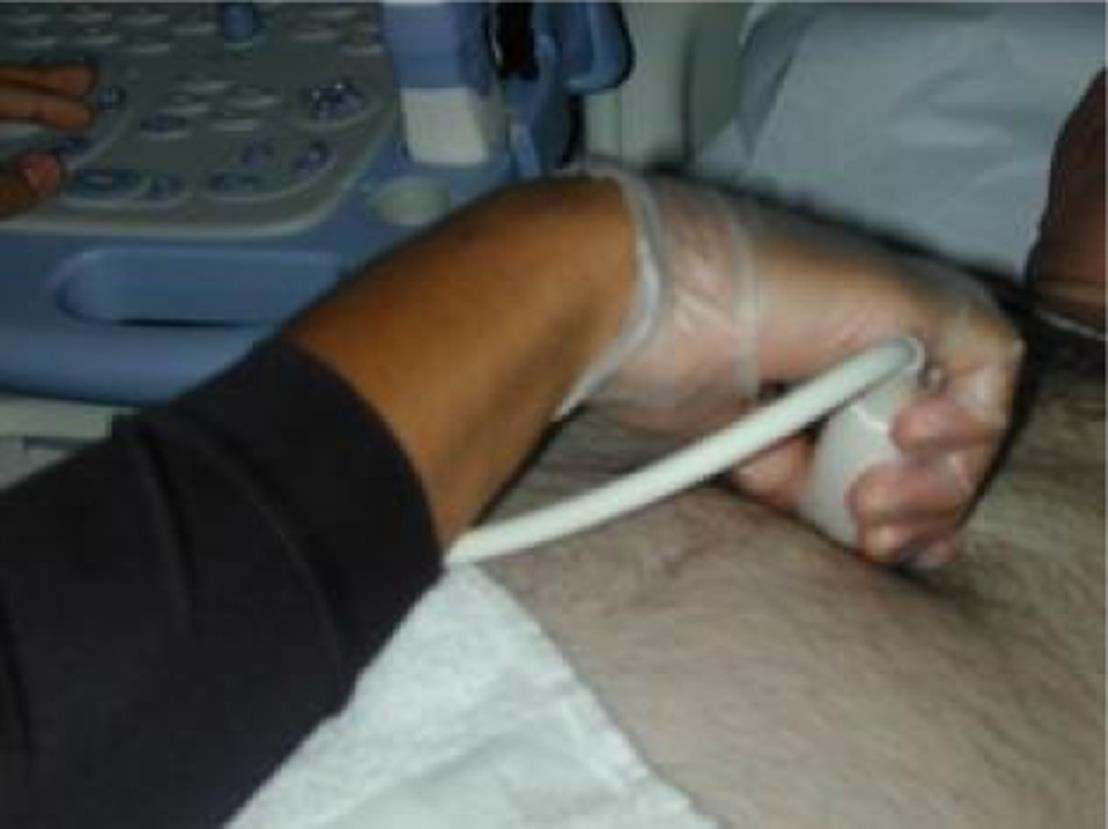
\includegraphics[width=\textwidth]{Figurer/wrist.jpg}
      \caption{Håndledsbøjning og greb om proben}
    \label{wrist}
  \end{minipage}
  \hspace{0.02\textwidth}
  \begin{minipage}{0.47\textwidth}
    \centering
      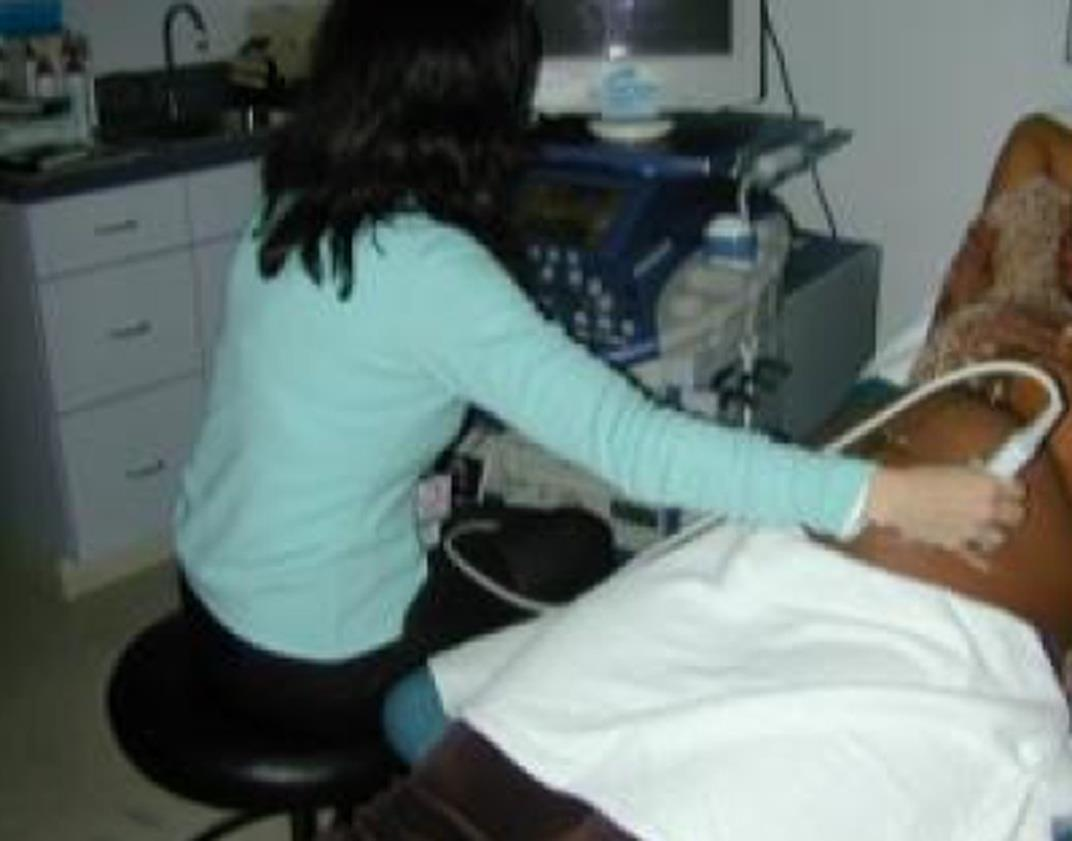
\includegraphics[width=\textwidth]{Figurer/arm.jpg}
      \caption{Arbejde i udstrakt arm}
    \label{udstraktArm}
  \end{minipage}
\end{figure}
Implementeringen af robotarmen vil føre til markante ændringer for sonografernes arbejdsstillinger. Disse ændringer kommer ved, at sonografen ikke længere skal sidde med armen ind over den gravide, og skaderne i skulderen vil derfor kunne undgås. Desuden vil sonografen være mere centreret omkring arbejdsstationen og derfor vil vrid i kroppen og nakken også blive mindsket. Sonografen skal dog stadig holde om dummy-proben, se under Teknologi \ref{Teknologi}, så den gribende belastning kan ikke fjernes helt. Men sammen med at de resterende belastninger kan mindskes eller helt fjernes, vil dette ikke have den samme belastende virkning. 


\subsection{Struktur}
På nuværende tidspunkt er den strukturelle opbygning på afdelingerne således, at en medarbejder ultralydsscanner henholdsvis 30 timer på HEH og 22 timer på RMV om ugen. De resterende timer udmønter sig som aflastende arbejde for den enkelte medarbejder. Denne struktur skyldes, at det er et kendt problem på afdelingerne, at scanningsarbejdet er fysisk belastende for medarbejderen. I løbet af en scanningsdag har én medarbejder i gennemsnit ti scanninger. Yderligere foretages der på afdelingerne forebyggende tiltag, i form af styrketrænende elastikøvelser, fri massage, ergonomiske redskaber samt fri adgang til fysioterapeuter og wellness-konsulenter, der kontrollerer og vejleder om medarbejderens arbejdsstillinger.

Afdelingerne tilrettelægger selv mængden af tid den enkelte sonograf skal scanne i løbet af en uge. Men Dansk Føtalmedicinsk Selskab udstikker hvert femte år anbefalinger, som det anbefales afdelingerne at følge. Anbefalingerne i forhold til antal timers ultralydscanning er 28 timer pr. uge, da det er vurderet at ved denne mængde af scanninger vil belastningen af sonografen ikke være i en skaden grad. (Mangler reference) Denne vurdering underbygges af videnskabelige forskningsundersøgelser, hvor sonografers arbejdsskader og mængden af scanningstid er blevet sammenholdt. Disse undersøgelser viser yderligere at en arbejdsskade typisk først optræder efter 5 år, hvilket der skal tages højde for i valget af observationsgruppe til lignende undersøgelser \cite{35}.
Dette viser, at RMV følger anbefalingen, mens HEH har sat niveauet 8 timer om ugen højere. Årsagerne hertil kan være flere, men typisk er at normeringerne og bevillingerne i forhold til antal sonografer og antallet af scanninger der skal udføres ikke gør det muligt at tilpasse arbejdsforholdet til anbefalingerne. 

Implementering af robotarmen vil føre til en ændring i afdelingernes strukturelle opbygning. Grundet at robotarmen vil gøre scanningsarbejdet væsentlig mindre belastende, og dermed vil det kunne føre til at en medarbejder vil kunne scanne fuldtids, altså 37 timer om ugen. Præcis hvilke arbejdsstillinger der er nu og hvilke det vil ændre sig til er beskrevet i afsnittet Aktør, Organisation. Fuldtids scanning vil føre til at de opgaverne sonograferne varetager som aflastende arbejde, vil skulle varetages af andet personale. Yderligere vil det føre til en ændring i antallet af sonografer der er behov for på den enkelte afdeling.

\subsection{Kultur}
Kulturen på HEH og RMV er meget teknologivenlig. Derfor formodes det, at implementeringen af teknologien ikke vil føre til væsentlige problemer i forhold til at få personalet til at benytte den nye teknologi. Dog kræves det, at der tilrettelægges en ordentlig plan for oplæring af personalet i brugen af teknologien. Personalet har generelt en god holdning og tillid til teknologi og er åbne for en mulig implementering af Ultralyds Robotarmen.

HEH har allerede på nuværende tidspunkt indvilliget i at være testafdeling for Robotic Ultrasound ApS under udviklingen af produktet. Det er i afdelingen interesse, da de ser en fremtid i produktet og dermed ønsker at være med til at tilpasse produktet til afdelingens struktur og behov.   

\section{Delkonklusion}

